\newpage
\section{Our Experiment}
\subsection{Infrastructure}
\paragraph{}As the experiment's infrastructure we will describe the frameworks used during the implementation. The framework that has been used to implement the item-based algorithm was Apache Spark. Also the ALS algorithm was used from the Apache Spark's MLLib library. The framework is common to infrastructure because Apache Spark can orchestrate the work on multiple machine as well as in one. So the framework is the closest you can get to the infrastructure.

\subsubsection{Apache Spark}
\paragraph{}The last decade, analyzing big data is at its peek. Lots of data are produced on daily basis. This means that the need of extracting information from them is raised. 
Lots of frameworks has been used in order to manage and analyze this amount of data. One of the analysis reasons is the need for accurate item recommendations to users. Those items could be movies (e.g. Netflix), music (e.g. Spotify) or products in general(e.g. Amazon). The one of the most popular frameworks that could enable this in a distributed way was Apache's Hadoop MapReduce.


\paragraph{}Apache Hadoop has also discrete jobs of processing data. The most common jobs are map and reduce but it has two more jobs, combine and partition. Hadoop has a master node and N worker nodes. The first is responsible to distribute the work, and the second for the work to be done. Each worker usually is called after the job is executing. Hence we have the mapper, the reducer, the partitioner and the combiner. In order to put this to a schema, you can see the figure \ref{hadoopJobsOrder} below.

\begin{figure}[h]
	\centering
	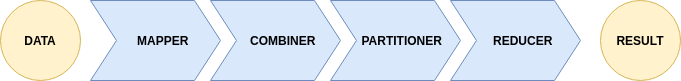
\includegraphics[width=0.5\textwidth]{images/HadoopMapReduceProcesses.png}
	\caption{\bfseries Hadoop Jobs Order}
	\label{hadoopJobsOrder}
\end{figure}

\paragraph{}Hadoop map reduce, is a distributed map-reduce system, 
this means that it has a mechanism to distribute work on nodes 
and a common interface for handling data. In Hadoop's case this was able to happen due to Apache Hadoop Yarn and the Hadoop Distributed File System or as commonly used HDFS. When a job was scheduled, data were loaded by the HDFS to a worker, 
then the worker was done, he was putting the result back to the HDFS. 

\paragraph{}As mentioned in \cite{ibmMapReduce:5}, "The term MapReduce actually refers to two separate and distinct tasks that Hadoop programs perform. The first is the map job, which takes a set of data and converts it into another set of data, where individual elements are broken down into tuples (key/value pairs). The reduce job takes the output from a map as input and combines those data tuples into a smaller set of tuples. As the sequence of the name MapReduce implies, the reduce job is always performed after the map job."

\paragraph{}So Hadoop has two basic processes, Map which is responsible for turning the data into key value pairs, and Reduce which takes those pairs and turns them into valuable data.

\paragraph{}If we would like to see where in the DIKW (Data Information Knowledge Wisdom) stack. The Map process would with data and the reduce will end up with information. Of course this in not always the case, lots of algorithms require lots of cycles in order to complete.
 
\begin{figure}[h]
	\centering
	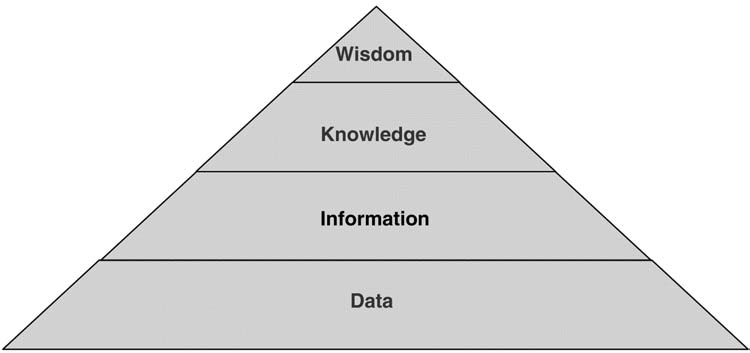
\includegraphics[width=0.5\textwidth]{images/DIKW.png}
	\caption{\bfseries Data Information Knowledge Wisdom Pyramid \cite{TheWisdomHierachy:7}}
	\label{dikw}
\end{figure}
% %note spark version
\paragraph{} But lets make a step back and take a look at Hadoop's architecture. As it is described in its official website \cite{Hadoop:9}, and shown in the figure \ref{hadoopStack} Hadoop uses Hadoop yarn in order to coordinate which process will run on which machine. Also it uses, its file system, the HDFS in order to have a common reference for the files over the network. Last but not least, Hadoop ecosystem is supported by the Hadoop Commons library. 

\begin{figure}[h]
	\centering
	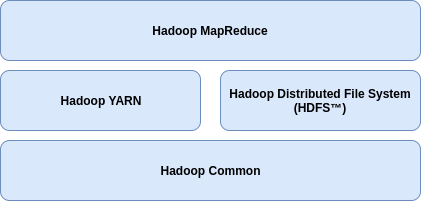
\includegraphics[width=0.5\textwidth]{images/hadoop-stack.png}
	\caption{\bfseries Hadoup Software Stack}
	\label{hadoopStack}
\end{figure}

\paragraph{} In 2009, University of California, Berkley, proposed a new framework for cluster computing in their paper, Spark: Cluster Computing with Working Sets \cite{Zaharia:2010:SCC:1863103.1863113}. They wanted to tackle two major Hadoop issues. 

\paragraph{}The first was the iterative jobs. Each Hadoop job reads from the disk to load data. This means that having iterative jobs, on any given algorithm, you were going to get a large time penalty on reading and of course writing to the disk. 

\paragraph{}The second issue was the interactive analytics. Each Hadoop SQL interface was running as a seperete job, and as we mentioned previously we have a big impact on execution time.

\paragraph{}In order to break the acyclic nature of Hadoop, they introduced the Spark's major abstraction, the RDDs. The name RDD stands for Resilient Distributed Datasets. Those datasets are a read-only collection of objects distributed across machines. If a machine fail, the lost part of the RDD can be recalculated. This notion is called lineage.

\paragraph{}Spark is implemented in Scala. Scala is a high-level statically typed programming language. At the time that paper was published it was believed that Spark was the only system available in a general purpose programming language to make clusters process large amount of data. As it was mentioned in \cite{Zaharia:2010:SCC:1863103.1863113} "We believe that Spark is the first system to allow an efficient, general purpose programming language to be used interactively to process large datasets on clusters"

\paragraph{}Back to RDDs, an RDD can be created with four different operations as it is described in \cite{Zaharia:2010:SCC:1863103.1863113}. The first operation is loading data from any shared file system. That file system could be HDFS or even an Amazon S3. The second way to create a RDD is by parallelizing any Scala collection. Spark will slice the collection into pieces and distribute it among the nodes. The third way is via transforming an RDD to another one. Because RDDs are immutable, any transformation operation on a RDD, filter, map, flatmap, will generate a new RDD. The last but not least method is by changing an RDDs persistence using save or cache operations.

\paragraph{}Spark also give us the power to do a lot of different distributed operations. Some of them was mentioned before, but we also have operations that would return data to the driver program like collect or reduce. 

\paragraph{}Another important feature of Sparks spine are the shared variables. Spark at its first appearance introduced two of them. The first shared variable is the broadcasted variables. Those variable, RDDs or not, are variables that are commonly used in an algorithm, like a look-up table. By broadcasting a variable, each node gets a copy of the variable in order to access it quickly. The second shared variable that was introduced in that paper was the Accumulators. Those variable live on the spark context, but they can only be increased by any worker and be read from the driver program only. That paper concludes that Spark can outperform Hadoop in some machine learning algorithms and more specific on logistic regression.

\begin{figure}[ht]
  \centering
    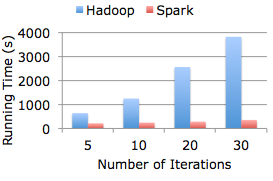
\includegraphics[width=0.5\textwidth]{images/hadoopVsSpark.png}
    \caption{\bfseries Logistic regression, Hadoop vs Spark \cite{HadoopVsSpark}}
   \label{hadoopVsSpark}
\end{figure}

\paragraph{}Coming back to today, Spark's current architecture is depicted below in fig. \ref{apacheSparkStack}.
Apache Spark was by design meant to work within Hadoop ecosystem, and most importantly with the HDFS. Apache Spark does not has a file system by itself. You can load data from almost any database, cloud-based or not, even from a local file system. But most will agree that Hadoop and Spark work together just perfect.

\begin{figure}[ht]
  \centering
    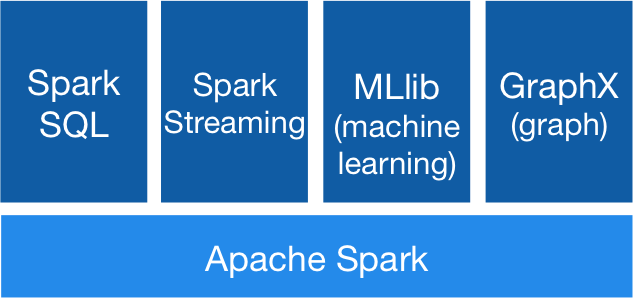
\includegraphics[width=0.5\textwidth]{images/spark-stack.png}
    \caption{\bfseries Apache spark stack \cite{ApacheSpark:1}}
   \label{apacheSparkStack}
\end{figure}

\paragraph{Notes:}
How spark differentiates from its predecessors\\
Spark lightweight in memory data transformation 
Resilient Distributed Datasets (RDDs) \\
mllibs\\
add spark jira note \\\\
Important note: mention als distributed broadcasting implementation. 
\\\\
When a RDD is been broadcasted in Apache Spark, this RDD becomes a local matrix to each machine. This means that you can use it for local calculations. This adds an overload to each machine depending on RDD's size. But it eliminates the network usage.
//cite the mastering apache spark book
\cite{ApacheSpark:1} \\
a Spark cluster to be created on AWS EC2 storage.\\
New trends on spark https://github.com/apache-spark-on-k8s/spark cite this repository too.
\subsection{Dataset}
\paragraph{}What is the dataset about. This dataset contains users, movies and the rating user made about the movies.
This dataset is splited to multiple subsets of 80000 training sets and respective 20000 reviews.
This dataset has been used by the related work on .....
\cite{MovieLens:3}

\subsection{Implementation and assumptions}
\paragraph{}During the implementation I had to make some assumptions and choices. The first of choices was the framework and the programming language that the implementation would take place. The framework that has been chosen, as you may had already figured out, is apache spark due to its trend and the high scalability it offers. The language of choice was scala, due to its functional nature.
\subsection{Metrics}
\paragraph{}After the implementation I had to make the choice of the metrics I was going to use.
\subsubsection{Mean Absolute Error}
\paragraph{}As metrics are commonly used the MSE, RMSE and MAE. Due to the fact that the author prefers the last one, MAE was used in this experiment.
\begin{equation}
MAE = \frac{\sum_{i=1}^{n}{|y_{i}-x_{i}|} }{n} = \frac{\sum_{i=1}^{n}\sqrt{{(y_{i}-x_{i})}^{2}}}{n}
\end{equation}
\subsubsection{Execution Time}
\paragraph{}Time is measured in milliseconds.
Execution time is always a measure when we are comparing algorithms. 
Even more if those algorithms execution time is heavily dependent to their complexity and not their resources.